\section{Diseño}

\subsection{Visión global de la aplicación}

\quad La aplicación consta de tres escenas:\\

\begin{itemize}
	\item Init: donde la aplicación empieza.
	\item EchoChamber: donde se testeará el efecto del eco.
	\item Forest: donde se prueba el efecto del 8D con varios focos de sonido.
\end{itemize}

\subsection{Escenas}
	\subsubsection{Init}
\quad Esta escena pretende poner en situación al usuario, indicando con un texto sobre una pared invisible como moverse y que es lo que tiene que hacer en ella.\\

\quad El objetivo será tan simple como encontrar el foco de sonido que lo está llamando. La voz para el foco ha sido aportada por Juan Hernández García, persona que menciono en los agradecimientos.\\

\begin{figure}[htb]
	\centering
	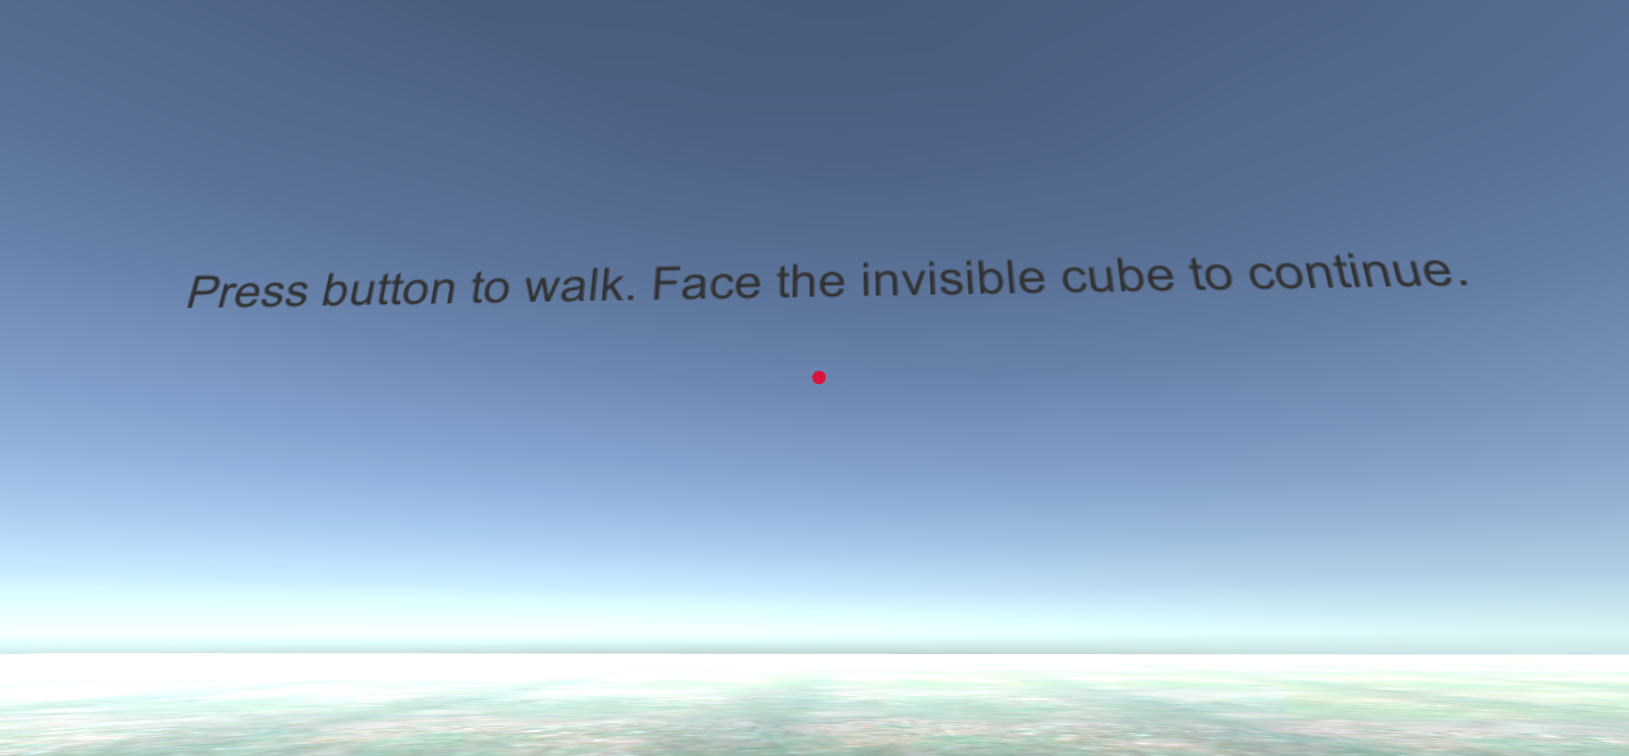
\includegraphics[width=0.6\textwidth]{./imagenes/initInstructions}
	\caption{Instrucciones de uso}
\end{figure} 

\begin{figure}[htb]
	\centering
	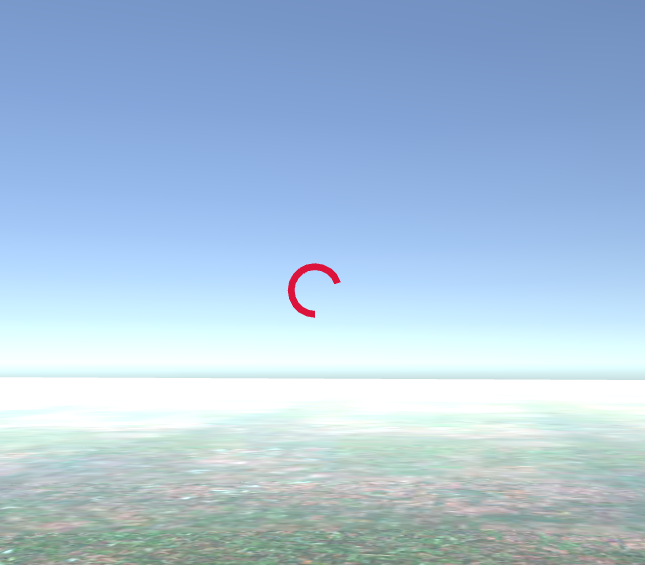
\includegraphics[width=0.248\textwidth]{./imagenes/inactiveCube}
	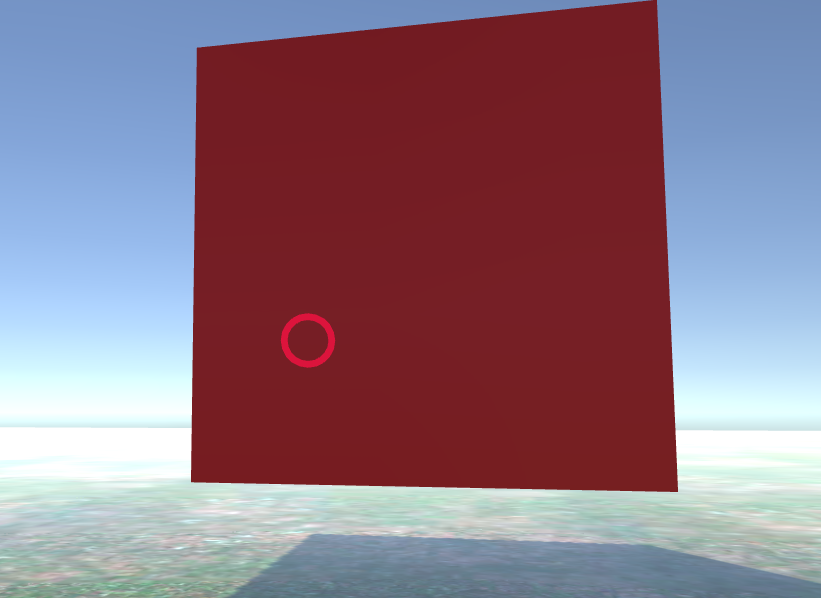
\includegraphics[width=0.3\textwidth]{./imagenes/activeCube}
	\caption{Cubo}
\end{figure} 

	\subsubsection{EchoChamber}
\quad Esta habitación tiene como objetivo mostrar el efecto del eco ante un foco de sonido, en este caso será un icosaedro que toca la tonadilla libre de derechos \textit{If i had a chicken}, típica canción de traberna del oeste. Este icosaedro se teletransportará a otro lugar de la habitación cuando interactuemos con él.\\

\begin{figure}[htb]
	\centering
	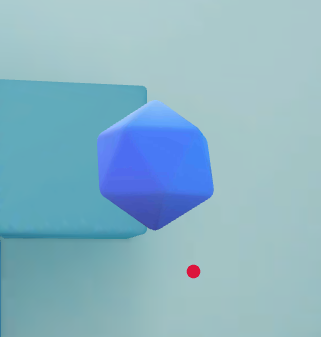
\includegraphics[width=0.4\textwidth]{./imagenes/icosaedroInactivo}
	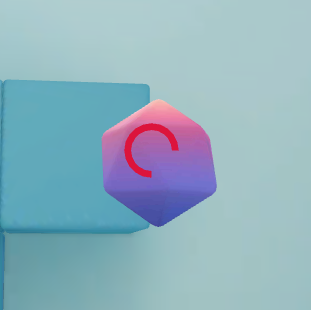
\includegraphics[width=0.4229\textwidth]{./imagenes/icosaedroActivo}
	\caption{Icosaedro sonoro}
\end{figure} 

\quad Además, se encontrarán dos menús, unos con dos botones y otro con varios desplegables.\\

\quad Mediante el menú de dos botones se podrá salir de la aplicación o avanzar a la última escena. Además este menú contará con un texto que indique la utilidad de esta escena.\\

\begin{figure}[htb]
	\centering
	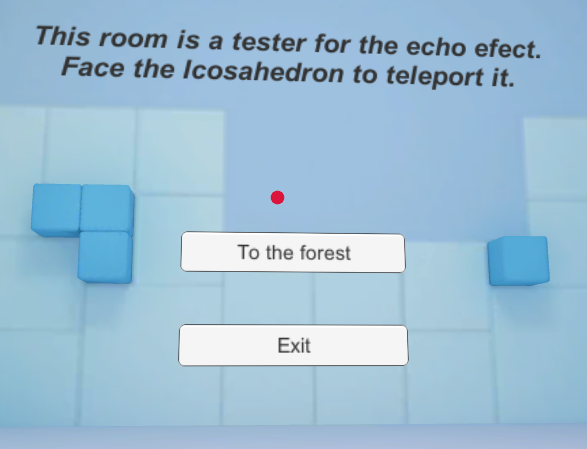
\includegraphics[width=0.5\textwidth]{./imagenes/echoMenu}
	\caption{Menú e instrucciones de la habitación}
\end{figure} 

\quad El menú de desplegables se utiliza para para cambiar el tipo de material del que se componen las supeficies de la habitación.\\ 

\begin{figure}[htb]
	\centering
	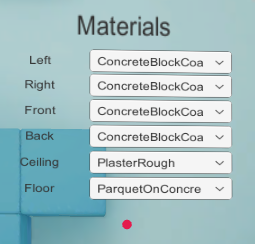
\includegraphics[width=0.3\textwidth]{./imagenes/materialMenu}
	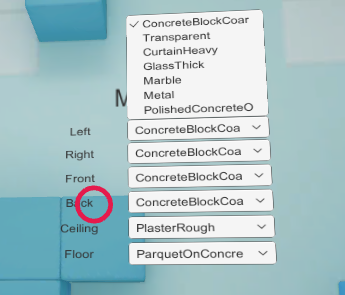
\includegraphics[width=0.4\textwidth]{./imagenes/materialMenuDeploy}
	\caption{Menú para cambio de materiales}
\end{figure} 
	
	\subsubsection{Forest}

\quad Esta escena pretende representar un pequeño bosque lleno de pajaros que van cantando, volando por las cercanías.\\

\quad Dispone de un menu para volver a la escena EchoChamber o salir de la aplicación.\\

\begin{figure}[htb]
	\centering
	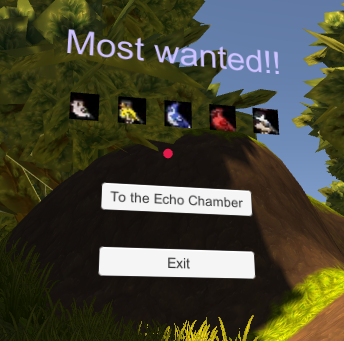
\includegraphics[width=0.36\textwidth]{./imagenes/forestMenu}
	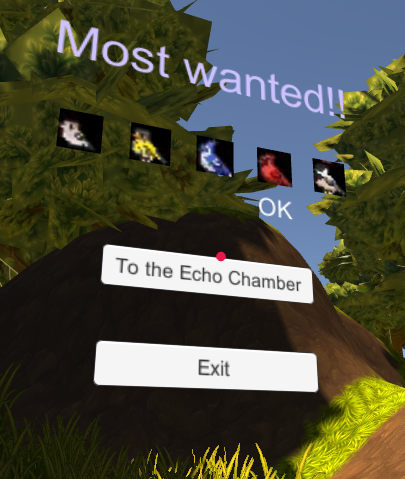
\includegraphics[width=0.30\textwidth]{./imagenes/forestMenuActive}
	\caption{Menú en el bosque}
\end{figure}

\quad En la parte superiro del menú se encuentra un banner con los cinco pajaros dentro de la selección que se introduzcan en la aplicación. Cuando se visualice al tipo de pájaro objetivo, se marcra en ese banner.\\

\begin{figure}[htb]
	\centering
	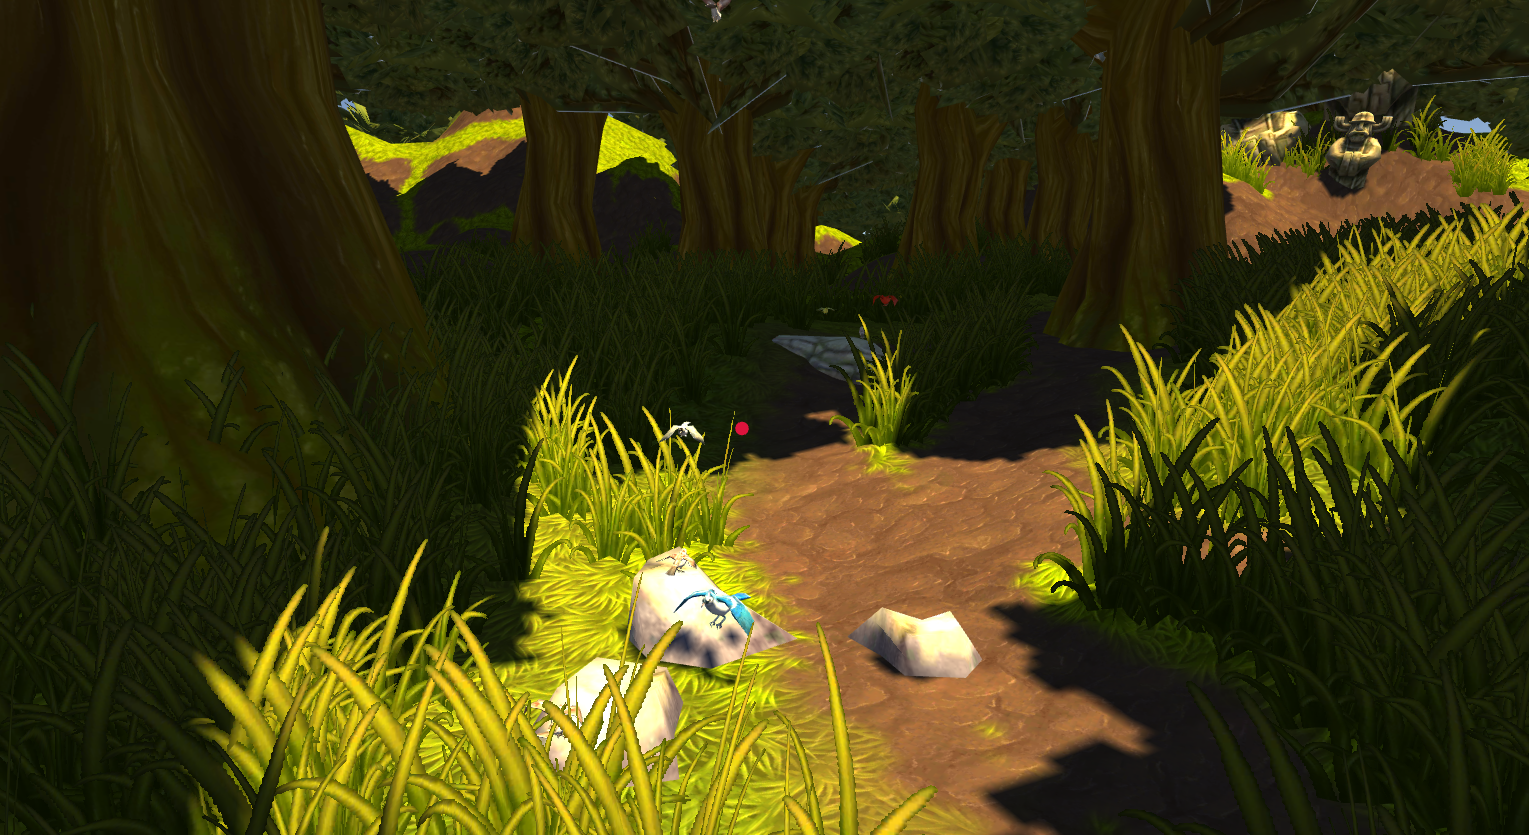
\includegraphics[width=0.7\textwidth]{./imagenes/forestBirds}
	\caption{Pajaros en el bosque}
\end{figure}

\quad Debido a la carga que tendrá esta escena, es importante cambiar shaders y aplicar técnicas de optimización para evitar que la tase de frames caiga demasiado.

\begin{figure}[htb]
	\centering
	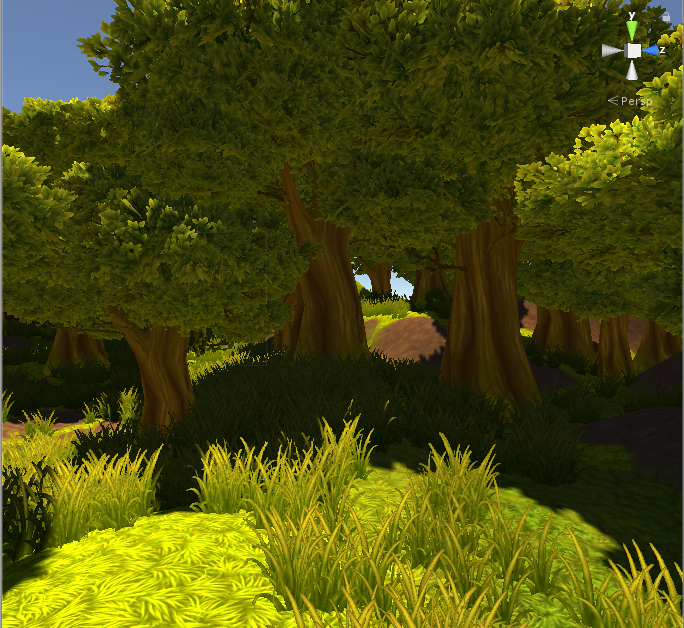
\includegraphics[width=0.45\textwidth]{./imagenes/highShadders}
	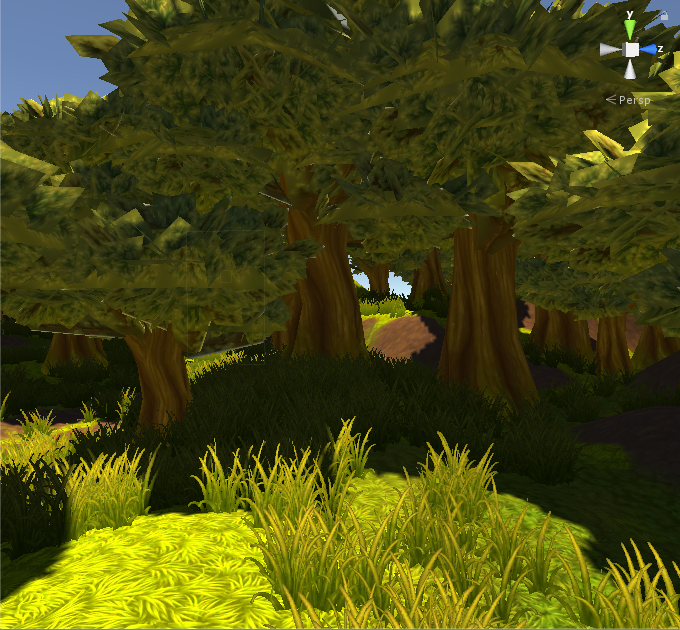
\includegraphics[width=0.45\textwidth]{./imagenes/lowShadders}
	\caption{Comparativa entre shader de alta calidad y baja calidad}
\end{figure}


\newpage


